\subsection{Internationalization}
\setauthor{Raffeiner Christine}
\begin{lstlisting}[language=HTML, caption=Internationalization-Makierung im HTML, label=lst:Internationalization_HTML]
  <mat-label i18n="label text|Question text">Fragetext eingeben</mat-label>
  <mat-card-title i18n="Title|card title" >Frage {{administration.question.sequenceNumber}}</mat-card-title>
\end{lstlisting}

Texte, die eine Übersetzung bekommen sollen, werden mit der Kennzeichnung i18n versehen, kurz für Internationalization.
Nach der Kennzeichnung können noch zusätzliche Informationen in der Form von i18n=\dq <Bedeutung> | <Beschreibung>\dq  für die automatische Übersetzung angegeben werden. 
In diesem Beispiel wurde keine automatische Übersetzung verwendet, trotzdem wurden zusätzliche Attribute angeben um im Falle eines Umstiegs schneller wechseln zu können.
\newline
\newline
\begin{lstlisting}[language=XML, caption=xliff-Datei, label=lst:xliffDatei]
  <?xml version="1.0" encoding="UTF-8" ?>
  <xliff version="1.2" xmlns="urn:oasis:names:tc:xliff:document:1.2">
  <file source-language="en" datatype="plaintext" original="ng2.template">
    <body>
      <trans-unit id="3292363768460657245" datatype="html">
        <source>Richtige Antwort</source>
        <target>Right Answer</target>
        <context-group purpose="location">
          <context context-type="sourcefile">src/app/answer-option-erstellen/answer-option-erstellen.component.html</context>
          <context context-type="linenumber">7</context>
        </context-group>
        <note priority="1" from="description">right answer</note>
        <note priority="1" from="meaning">checkbox text</note>
      </trans-unit>
      <trans-unit id="878423452191694276" datatype="html">
        <source><x id="INTERPOLATION" equiv-text="{{this.questions.length}}"/> Fragen</source>
        <target><x id="INTERPOLATION" equiv-text="{{this.questions.length}}"/> Question</target>
        <context-group purpose="location">
          <context context-type="sourcefile">src/app/answer-survey/answer-survey.component.html</context>
          <context context-type="linenumber">4</context>
        </context-group>
        <note priority="1" from="description">qestion anz</note>
        <note priority="1" from="meaning">headline text</note>
      </trans-unit>
      ...
\end{lstlisting}

Durch die Ausführung des Befehls \textit{ng xi18n --output-path src\textbackslash locale} werden alle Texte mit dem Kennzeichen ibn18 in eine XLF-Datei
extrahiert. In der Datei wird zuerst angegeben in welcher Form sie geschrieben ist. In diesem Fall ist es eine XLF-Datei mit der Version 1.2 (Angular Standard). (Zeile 2)
\newline
\textit{source-language=\dq en\dq} gibt die Sprache an. (Zeile 3)
\newline
Eine \textit{<trans-unit>} wird für jeden mit einer Kennzeichnung versehenen Text generiert. (Zeile 5)
\newline
In \textit{<source>} steht der Originaltext, der angegeben wurde. (Zeile 6)
\newline
Der Text der nun als Übersetzung gilt muss umklammert von \textit{<target> <\textbackslash target>} für jede \textit{<trans-unit>} selbst übersetzt und unter \textit{<source>} eingefügt werden. (Zeile 7)
\newline
\newline
\begin{lstlisting}[language=TypeScript, caption=Konfigurieren der Sprachen im angular.json, label=lst:Angular.json]
  "i18n": {
    "sourceLocale": "de",
    "locales": {
      "en": "src/locale/language_source.eng.xlf"
      }
    ...
    "en":{
    "localize": ["en"]
     },
    "de":{
      "localize": ["de"]
    },
    ...
\end{lstlisting}
Zum Schluss muss der Applikation noch mittgeteilt werden, wo die Ausgangssprache Datei liegt (Zeile 4) und in welcher Sprache diese angegeben ist. 
Zeile 7 und 10 sind Kürzel, die später für das Starten der Applikation wichtig sind.
\newline
\newline
Es ist zu beachten, dass nach diesen Änderungen beim Starten der Applikation immer anzugeben ist welche Sprache verwendet werden soll.
Beispielsweise: \textit{ng serve --configuration=de} oder \textit{ng serve --configuration=en}
Durch kleine Änderungen im package.json kann auch automatisiert eine bestimmte Sprache gestartet werden.

\begin{lstlisting}[language=TypeScript, caption=automatisches Starten der deutschen Sprache, label=lst:package.json]
  "scripts": {
    "ng": "ng",
    "start": "ng serve --configuration=de",
    ...
\end{lstlisting}
Mittels \textit{npm start} wird nun automatisch die deutsche Version der Applikation gestartet.

\subsection{Angular-CSS bearbeiten}
\setauthor{Raffeiner Christine}
\begin{lstlisting}[language=TypeScript, caption=Semi-Transperentes Eingabefeld, label=lst:Ng-deep]
::ng-deep .mat-form-field-appearance-fill .mat-form-field-flex {  
    background: rgba(255, 255, 255, 0.5);
}
\end{lstlisting}
Um den Hintergrund einer Material-Komponente Mat-Form-Field (eine Komponente die Formularelemente
einschließt) halbtransparent zu machen wurde ng-deep verwendet.
\newline
\newline
Ng-deep ermöglicht den Zugriff auf DOM-Elemente, in nicht selbstgeschriebenen Komponenten.
Im Beispiel von Angular Material (oder eine andere Bibliothek eines Drittanbieters wie Materials), befinden 
sich die Elemente außerhalb des Bereichs (wie zum Beispiel Eingabefelder), und lassen keinen direkten Zugriff mit CSS auf diese Elemente 
zu. Ng-deep ermöglicht diesen Zugriff. Mehr Infos zu Angular Material befinden sich im Kapitel \ref{chap:materials}.

\subsection{Keycloak}
\setauthor{Raffeiner Christine}
Mittels des Keycloak können sich die Benutzer der Applikation mit gewohnten Anmeldeinformationen anmelden.
\begin{lstlisting}[language=TypeScript, caption=Konfiguration des Keycloaks, label=lst:Konfiguration-Keycloak]
{
  "backendApiUrl": "http://localhost:8080/api",
  "keycloakUrl": "http://localhost:8180/auth/realms/School"
}
\end{lstlisting}
Für die Anbindung des Keycloaks an das Frontend muss zuerst festgelegt werden, unter welcher URL sich der KeycloakService und das Backend befinden.
\newline
\newline
\begin{lstlisting}[language=TypeScript, caption=Aufrufen des Logins, label=lst:Initialisierung Login]
  openLogin(){
    this.config.init().then(() => this.authenticationService.initializeLogin())
  } 
\end{lstlisting}
Wird nun das Login aufgerufen wird der Authentifikations-Service initialisiert.
\newline
\newline
\begin{lstlisting}[language=TypeScript, caption=Initialisierung des AuthenticationService, label=lst:authenticationService]
  init(): Promise<any> {
    return this.httpClient
      .get<Config>('/assets/config.json')
      .pipe(
        tap(config => {
          this.config = config;
          authModuleConfig.resourceServer.allowedUrls!.push(config.backendApiUrl);
        })
      )
      .toPromise();
  }
\end{lstlisting}
Mit der Initialisierung werden die angegebenen Konfigurationsdateien ausgelesen und die angegeben URLs zum Weiterleiten zugelassen.
\newline
\newline
\begin{lstlisting}[language=TypeScript, caption=Aufrufen des Authentifikationswächters, label=lst:URLRouten]
  const routes: Routes = [
    {path: '', component: StartseiteComponent, pathMatch: "full"},
    {path: '', canActivateChild: [AuthGuard], children: [
      //{path: '', redirectTo: '/dashboard', pathMatch: 'full'},
      {path: 'dashboard', component: DashboardComponent},
      {path: 'fragebogen-erstellen', component: FragebogenErstellenComponent},
      {path: 'dashboard/fragebogen-editieren/:id', component: EditQuestionnaireComponent}
    ]},
    {path: 'answerSurvey', component: AnswerSurveyComponent},
    {path: 'startseite', component: StartseiteComponent},
    {path: '**', component: StartseiteComponent}
  ];
\end{lstlisting}
Man wird nicht nur mit dem Klick auf den Login-Knopf zum Anmelden auf den Keycloak weitergeleitet. Will man auf 
Unterseiten, die einen Login erfordern zugreifen, wird man ebenfalls automatisch zum Login weitergeleitet. Dies wird mittels 
Authentifikationswächtern (authentificationguards) bewerkstelligt. In diesem Fall wird der Wächter aufgerufen, wenn auf 
jede Unterseite (Zeile 3, 4, 5, 6 und 7) (bis auf die Startseite und die Seite zum Beantworten der Fragen (Zeile 9 und 10)) aufgerufen wird.
\newline
\newline
\begin{lstlisting}[language=TypeScript, caption=Authentifikationswächter, label=lst:Authentifikationswächter]
  canActivateChild(
    childRoute: ActivatedRouteSnapshot,
    state: RouterStateSnapshot
  ): Observable<boolean | UrlTree> | Promise<boolean | UrlTree> | boolean | UrlTree {
    console.log(this.authenticationService.oidcLoaded.value);
    if (this.authenticationService.oidcLoaded.value) {
      return true;
    }
      this.config.init().then(() => this.authenticationService.initializeLogin())
      return false;
  }
\end{lstlisting}
Der Authentifikationswächter überprüft beim Aufrufen einer Seite, die er überwacht beziehungsweise beschützt, ob der 
derzeitige Benutzer sich bereits einmal angemeldet hat (Zeile 6). Sollte das der Fall sein wird der Benutzer auf die gewünschte Seite weitergeleitet. 
Hat sich der Benutzer noch nicht eingeloggt wird der Authentifikations-Service initialisiert und der derzeitige Aufrufen der Unterseite abgewiesen. (Zeile 9 und 10) 
\newline
\newline
\begin{lstlisting}[language=TypeScript, caption=Login und Logout, label=lst:Login und Logout]
  username = new BehaviorSubject<string>('');
  roles = new BehaviorSubject<string[]>([]);
  oidcLoaded = new BehaviorSubject<boolean>(false);
  ...
  logOut() {
    this.oAuthService.logOut();
  }
  
  async initializeLogin(): Promise<void> {
    console.log(this.configService.config);
    this.oAuthService.configure({
      issuer: this.configService.config.keycloakUrl,
      redirectUri: window.location.origin,
      clientId: 'my-frontend-service',
      responseType: 'code',
      scope: 'offline_access',
      showDebugInformation: true
    });
    await this.oAuthService.loadDiscoveryDocumentAndTryLogin({
      customHashFragment: window.location.search
    });
  
    if (!this.oAuthService.hasValidAccessToken()) {
      this.oAuthService.initLoginFlow();
    } else {
      this.oAuthService.setupAutomaticSilentRefresh();
      const profile: any = await this.oAuthService.loadUserProfile();
      this.username.next(profile.info.preferred_username)
      this.roles.next(this.parseJwt(this.oAuthService.getAccessToken()).realm_access.roles);
      this.oidcLoaded.next(true);
    }
  }
\end{lstlisting}
Mit dem Aufruf der Logout-Methode wird der Authentifikations-Service benachrichtigt und loggt den Benutzer aus. (Zeile 1 und 2).
Will sich der Benutzer nun einloggen, werden zuerst einige wichtige Informationen gesetzt wie zum Beispiel der Name des Client des Keycloaks 
für die Applikation (Zeile 10) und wo der Benutzer nach erfolgreichem Einloggen, hingeleitet wird (Zeile 9). Ist der 
Benutzer nicht eingeloggt wird der Benutzer zum Login über den Keycloak weitergeleitet. (Zeile 20). 
Ist der Benutzer bereits eingeloggt wird der Authentifikations-Token erneuert und der Benutzername und die Rolle aktualisiert.
\newline
\newline
Das Erhalten der Anmeldedaten wurde mithilfe eines Observable-Patterns gelöst. Daten können hierbei in ein Oberservable gegeben werden.
Ändern sich die Daten des Oberservables werden die Observer, die das Oberservable beobachten, benachrichtigt.
\newline
\newline
Nach erfolgreichem Login werden die Anmeldedaten in ein Oberservable gegeben - konkret in ein BehaviorSubject, das als Oberservable 
fungiert. Um die Daten zu erhalten, wird ein Subscribe auf das BehaviorSubject durchgeführt.
\newline
\newline
\begin{lstlisting}[language=TypeScript, caption=Verwendung der geschickten Daten TypeScript, label=lst:Verwendung der Anmeldedaten TypeScript]
  ngOnInit(): void {
    this.authenticationService.username.subscribe(value => {
      this.logged_in = (value.length > 1);
    })
  }
\end{lstlisting}
\begin{lstlisting}[language=html, caption=Verwendung der geschickten Daten HTML, label=Verwendung der Anmeldedaten HTML]
  ...
  <button *ngIf="!this.logged_in" i18n="button text|Login button text" mat-stroked-button color="primary" (click)="openLogin()">Einloggen</button>
  <div *ngIf="this.logged_in">
    <button mat-stroked-button color="primary" routerLink="/dashboard">Dashboard</button>
    <button i18n="button text|Logout button text" mat-stroked-button color="primary" (click)="loggoutUser()">Ausloggen</button>
  </div>
  ...
\end{lstlisting}
Der Header der Webseite führt beispielsweise ein Subscribe auf das BehaviorSubject, dass den Benutzernamen beinhaltet, aus. Ist der 
Benutzer nicht eingeloggt, ist beim Laden der Seite der Wert des BehaviorSubject leer. Daraufhin wird ein Login-Button angezeigt.
Loggt sich der Benutzer nun ein, wird der Observer des Headers darüber informiert und statt des Login-Buttons wird nun ein 
Logout-Button und ein Button der zum Dashboard führt angezeigt.

\subsection{CSV-Download}
\setauthor{Raffeiner Christine}
\begin{lstlisting}[language=TypeScript, caption=CSV-Download, label=lst:CSV-Download]
    const dialogRef = this.generateTransactionCodes.open(TransactionComponent,{width:"30%"});

    dialogRef.afterClosed().subscribe(result => {
      if((typeof result) == "number"){
        this.transactionservice.generateTransactioncodes(result, this.survey.id).subscribe((response : any)=>{
          let dataType = response.type;
            let binaryData = [];
            binaryData.push(response);
            let downloadLink = document.createElement('a');
            downloadLink.href = window.URL.createObjectURL(new Blob(binaryData, {type: dataType}));
            if ("transactionCodes.csv"){
                downloadLink.setAttribute('download', "transactionCodes_" + this.survey.title + ".csv");
                document.body.appendChild(downloadLink);
                downloadLink.click();
            }
        });
      }
    });
\end{lstlisting}
Es wird ein Dialogfenster geöffnet (Zeile 1) in dem die Anzahl der Transaktions Codes angegeben wird. Nach dem Schließen des 
Dialogfensters wird überprüft, ob das Dialogfenster \dq richtig \dq geschlossen wurde - es wurde eine Zahl angegeben 
und \textit{Generieren} und nicht \textit{Zurück} ausgewählt (Zeile 2 \& 3). Danach werden die Transactioncodes mittels 
einer HTTP-Anfrage an den Server generiert. Dieser schickt ein CSV-File an das Frontend zurück (Zeile 4). 
Die Daten werden von einem JSON-Objekt wieder in eine CSV-File umgewandelt (Zeile 5, 6 und 7) und danach wird das File 
zum Herunterladen bereit gemacht (8 und 9). Der Datei wird noch ein Name verliehen (Zeile 11) und danach automatisch heruntergeladen (DownloadLink wird geklickt Zeile 13).

\subsection{Reaktive Formulare}
\setauthor{Raffeiner Christine}
Reaktive Formulare werden für die Verarbeitung und Überprüfung von Formulareingaben verwendet.
\newline
\newline
\begin{lstlisting}[language=TypeScript, caption=Formularüberprüfung mit reakitven Formularen TypeScript, label=lst:Formularüberprüfung]
this.userForm = new FormGroup({
  name: new FormControl('', [Validators.required, Validators.minLength(5), Validators.maxLength(50)]),
  desc: new FormControl('', [Validators.required, Validators.minLength(5), Validators.maxLength(250)])
});
\end{lstlisting}
Um reaktive Formulare zu verwenden, muss eine \textit{FormGroup} (stellvertretend für das Formular) mit 1 oder mehreren 
Einträgen mit \textit{FormControl} (stellvertretend für eine Formulareingabe) erstellt werden. Die im \textit{FormControl} angegebenen Validationen dienen
zur Überprüfung, ob das Feld für den Gebrauch, richtig ausgefüllt worden ist. In diesem Fall sollen die Felder ausgefüllt und zwischen 5 und 50 \textbackslash  250 Zeichen enthalten.

\begin{lstlisting}[language=html, caption=Formularüberprüfung mit reakitven Formularen HTML, label=lst:impl:foo]
<form [formGroup]="userForm">
  ...
  <input matInput formControlName="name" i18n-placeholder="placeholder text|placeholder for questionnaire name" placeholder="Umfragename eingeben" name="questinnairename" [(ngModel)]="this.questionnaire.name" required>   
  <mat-error *ngIf="userForm.controls['name'].invalid">
  <p i18n="error message|error name">Name muss zwischen 5-50 Zeichen enthalten.</p>
...
\end{lstlisting}

Um die \textit{FormGroup} und die \textit{FormControl} mit den zugehörigen Elementen zu verknüpfen, müssen diese im HTML 
referenziert werden. (Zeile 1 und 3). Sollten die angegeben Validationen nicht erfüllt sein, wird ein entsprechender Fehlertext angezeigt. (Zeile 4)

\subsection{Berechnen der anzuzeigenden Fragen}
\setauthor{Raffeiner Christine}
Beim Beantworten von Fragen werden nur eine gewissen Menge an Fragen auf einmal angezeigt, um langes Scrollen zu 
verhindern. Zudem soll es den Benutzer / die Benutzerin dabei unterstützen sich immer nur auf ein paar Fragen zu fokussieren, um nicht überwältigt zu werden.
\begin{lstlisting}[language=html, caption=Pageinator, label=lst:Berechnen anzuzeigender Fragen HTML]
  ...   
  <div class="mat-paginator-container">
  <mat-paginator [showFirstLastButtons]="true" [length]="this.questions.length" [pageSize]="pageSizeOptions[1]" [pageSizeOptions]="pageSizeOptions" aria-label="Select page" (page)="recalc($event)">
  </mat-paginator>
  </div>

  <div id="questionsbox">
  <div *ngFor="let item of this.indexArray, let i=index">
    <app-questions-to-answer [questionToAnswer]="this.questionsToAnswer[item]"></app-questions-to-answer>
  </div>
  </div>
  ...
\end{lstlisting}
Während der Beantwortung der Fragen wird mit einem Pageinators gearbeitet, (Zeile 2) der die gesamten Fragen auf mehrere Seiten aufteilt. Dieser hilft dabei, die Fragen nur 
stückchenweise anzuzeigen. Mit ihm können die gesamte Anzahl an Fragen, die angezeigt werden 
(3, 5 oder 10 Fragen Standardmäßig wurde 5 eingestellt) und die Seite, die man ansteuern will, eingestellt werden.
Es ist auch möglich, schnell auf die erste und letzte Seite zu springen. Werden die Standardeinstellungen geändert oder wird die Seite gewechselt, werden die angezeigten Fragen neu berechnet. 
\newline
\newline
\begin{lstlisting}[language=TypeScript, caption=Berechnen der anzuzeigenden Fragen TypeScript, label=lst:Berechnen anzuzeigender Fragen HTML]
  ...
  recalc(pageEvent: PageEvent){
    this.fillArray(pageEvent.pageSize * pageEvent.pageIndex, pageEvent.pageSize * (pageEvent.pageIndex + 1));
  }
  
  fillArray(start : number, end : number){
    this.indexArray = [];
    for (let index = start; index < end; index++) {
      if(index < this.questionsToAnswer.length){
        this.indexArray.push(index);
      }
    }
  }
  ...
\end{lstlisting}
Für die Berechnung wird ein Event ausgelöst, welches mitteilt, dass sich die Einstellungen verändert haben (Zeile 2). 
Danach wird ein Array, mit den anzuzeigenden Fragen, zuerst geleert und danach befüllt.

\subsection{Konfiguration des Traefik}
Traefik wurde für die Sicherheit, genauer gesagt die Verwendung von https statt http eingesetzt.
HTTPS- und HTTP-Anfragen werden innerhalb des DockerContainer auf HTTP-Anfragen umgeleitet.
Zudem wurde eine festgelegte Version des Traefik-Images verwendet und ein Dashboard hinzugefügt (siehe \ref{fig:treafikDashboard}). 
\begin{lstlisting}[caption=Starten Traefik, label=lst:Traefik]
  version: "3.3"
  services:
    traefik:
      image: "traefik:v2.6"
      command:
        - --entrypoints.web.address=:80
        - --entrypoints.websecure.address=:443
        - --providers.docker
        - --api
      ports:
        - "80:80"
        - "8080:8080"
        - "443:443"
      volumes:
        - "/var/run/docker.sock:/var/run/docker.sock:ro"
      labels:
        # Dashboard
        - "traefik.http.routers.traefik.rule=Host(`traefik.docker.localhost`)"
        - "traefik.http.routers.traefik.tls.certresolver=leresolver"
        - "traefik.http.routers.traefik.service=api@internal"
        - "traefik.http.routers.traefik.entrypoints=websecure"
  
      # middleware redirect
        - "traefik.https.middlewares.redirect-to-http.redirectscheme.scheme=http"
  
      # global redirect to http
        - "traefik.https.routers.redirs.rule=hostregexp(`{host:.+}`)"
        - "traefik.https.routers.redirs.entrypoints=web"
        - "traefik.https.routers.redirs.middlewares=redirect-to-http"
\end{lstlisting}

\begin{figure}[H]
  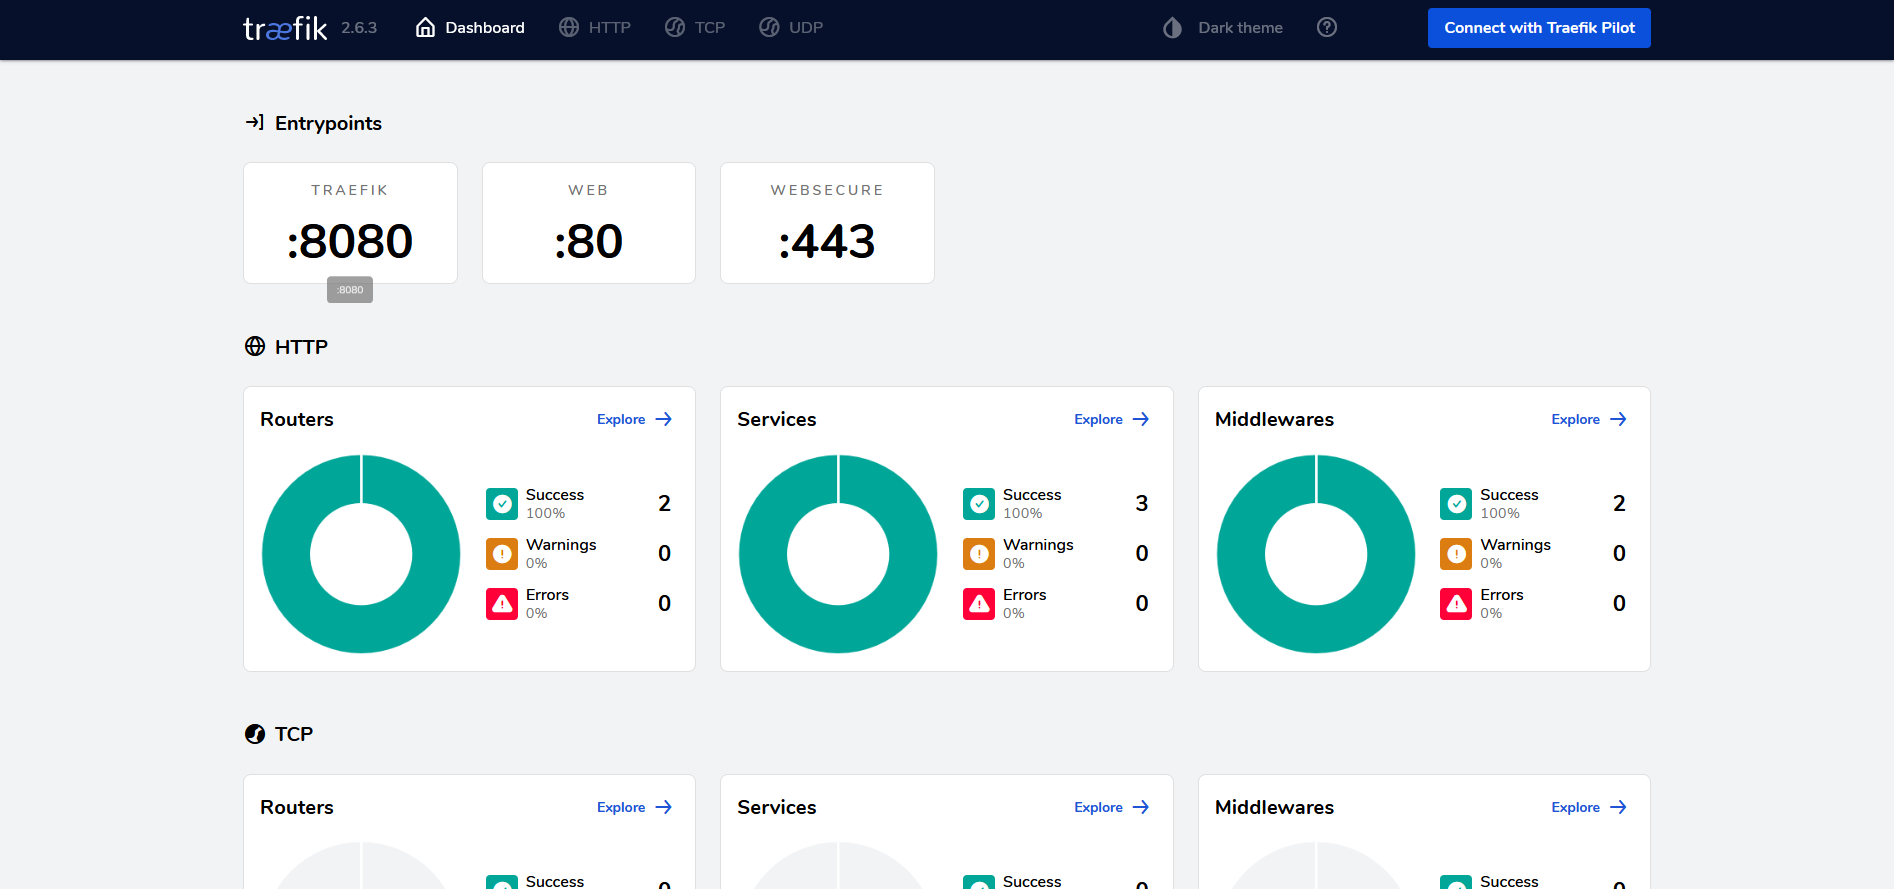
\includegraphics[width=0.8\textwidth]{pics/TreafikDashboard.PNG}
  \centering
  \caption{Dashboard Traefik}
  \label{fig:treafikDashboard}
\end{figure}

\subsection{Dockerfiles}
\subsubsection{Keycloak Docker}
\begin{lstlisting}[caption=Keycloak Dockerfile, label=lst:Dockerfile Keycloak]
version: '3.9'
services:
  keycloak:
  # Name des Containers
    container_name: keycloak
  environment:
    # Zugriffsdaten
      - KEYCLOAK_USER=admin
      - KEYCLOAK_PASSWORD=admin
    # Eingebaute h2 Datenbank
      - DB_VENDOR=h2
    ports:
      - '8180:8080'
    # Image auf dem Aufgebaut wird
    image: 'quay.io/keycloak/keycloak:15.0.2'
    volumes:
    # Speicherort der Zertifikate der Benutzer und Benutzerinnen  
      - ./certs:/etc/ssl/certs/java
    # Speicherort der Keycloak Standarteinstellungen
      - ./imports:/opt/jboss/keycloak/imports
    # Einlesen der Standardeinstellungen und Verhalten des Einlesens bereits vorhandene Objekte nicht ersetzeten
    command: [ '-b', '0.0.0.0', '-Dkeycloak.profile.feature.upload_scripts=enabled', '-Djavax.net.ssl.trustStore=/etc/ssl/certs/java/cacerts', '-Djavax.net.ssl.trustStorePassword=changeit', '-Dkeycloak.migration.action=import', '-Dkeycloak.migration.provider=singleFile','-Dkeycloak.migration.strategy=IGNORE_EXISTING' ,'-Dkeycloak.migration.file=/opt/jboss/keycloak/imports/keycloak_settings.json' ]
    networks:
      - keycloak_network

networks:
  keycloak_network:
    name: keycloak_network
    driver: bridge
\end{lstlisting}
Die importierten Standardeinstellungen erstellen automatisch das Realm, Clients für Frontend und Backend, die Rollen, etc. die 
für die Benutzung gebraucht werden. Somit müssen die Einstellungen nicht jedesmal beim Starten manuell ausgeführt werden.
\begin{lstlisting}[caption=Auszug aus den importieren Einstellungen, label=lst:Imortierte Einstellungen]
  {
    "id": "School",
    "realm": "School",
    "notBefore": 0,
    "defaultSignatureAlgorithm": "RS256",
    "revokeRefreshToken": false,
    "refreshTokenMaxReuse": 0,
    "accessTokenLifespan": 300,
    "accessTokenLifespanForImplicitFlow": 900,
    "ssoSessionIdleTimeout": 1800,
    "ssoSessionMaxLifespan": 36000,
    "ssoSessionIdleTimeoutRememberMe": 0,
    "ssoSessionMaxLifespanRememberMe": 0,
    "offlineSessionIdleTimeout": 2592000,
    "offlineSessionMaxLifespanEnabled": false,
    "offlineSessionMaxLifespan": 5184000,
    "clientSessionIdleTimeout": 0,
    "clientSessionMaxLifespan": 0,
    "clientOfflineSessionIdleTimeout": 0,
    "clientOfflineSessionMaxLifespan": 0,
    "accessCodeLifespan": 60,
    "accessCodeLifespanUserAction": 300,
    ...
\end{lstlisting}

\subsubsection{Postges Docker}
\begin{lstlisting}[caption=Postgres Dockerfile, label=lst:Postges Dockerfile]
  version: '3.1'
  services:
    # Datenbank
    db:
    # Containername
      container_name: survey_postgres
    # Image auf das Aufgebaut wird
      image: postgres:13.3-alpine
  
    # Bei (manuell oder anderweitigen) stoppen der DB wird, nicht neu gestartet wird, selbst wenn der Docker-Daemon neu startet
      restart: unless-stopped
    # Zugriffsdaten
      environment:
        POSTGRES_USER: postgres
        POSTGRES_PASSWORD: postgres
        POSTGRES_DB: db
      ports:
        - 5432:5432
      volumes:
      # Speicherort der permanenten Daten
        - ./db-postgres/db:/var/lib/postgresql/data
      # Importdatenspeicherort
        - ./db-postgres/import:/import
      networks:
        - postgres
  
    # grafische Tool zur Entwicklung und Administration
    pgadmin:
      container_name: survey_pgadmin
      image: dpage/pgadmin4:5.5
      environment:
        PGADMIN_DEFAULT_EMAIL: ${PGADMIN_DEFAULT_EMAIL:-pgadmin4@pgadmin.org}
        PGADMIN_DEFAULT_PASSWORD: ${PGADMIN_DEFAULT_PASSWORD:-admin}
        PGADMIN_CONFIG_SERVER_MODE: 'False'
      volumes:
        - ./db-postgres/pgadmin:/root/.pgadmin
      ports:
        - 8090:80
      networks:
        - postgres
      restart: unless-stopped
  
  networks:
    postgres:
      driver: bridge  
\end{lstlisting}

\subsection{Fragebogen duplizieren}
In dieser Diplomarbeit besteht die Möglichkeit, Fragebögen zu duplizieren. Dies wurde mit dem Code von
\ref{lst:duplicateQuestionnaire} umgesetzt. In diesem Code wird der übergebene Questionnaire ohne id in der Datenbank
gespeichert. Da damit aber nur der Fragebogen und nicht die Fragen oder die Antwortmöglichkeiten dupliziert wurde,
müssen die Questions und AnswerOptions gefunden werden, welche für den aktuellen Fragebogen verwendet werden.
Ist dies geschehen, werden auch diese Daten ohne id in der Datenbank gespeichert. Erst wenn das alles erfüllt ist,
wurde der Fragebogen richtig kopiert.
\begin{lstlisting} [caption=Fragebogen duplizieren, label=lst:duplicateQuestionnaire]
public Questionnaire duplicateQuestionnaire(Questionnaire questionnaire, Interviewer interviewer) {
  Questionnaire originalQuestionnaire = findQuestionnaire(questionnaire);
  Questionnaire duplicateQuestionnaire;
  duplicateQuestionnaire = new Questionnaire(
    originalQuestionnaire.name,
    originalQuestionnaire.description,
    false,
    interviewer);
  duplicateQuestionnaire = save(duplicateQuestionnaire);
  Question duplicateQuestion;
  List<Question> questions = questionRepository.findByQuestionnaire(originalQuestionnaire);
  AnswerOption duplicateAnswerOption;
  List<AnswerOption> answerOptions;
  for (Question originalQuestion : questions) {
    duplicateQuestion = new Question(
      originalQuestion.text,
      originalQuestion.sequenceNumber,
      originalQuestion.questiontype,
      duplicateQuestionnaire);
    duplicateQuestion = questionRepository.save(duplicateQuestion);
    answerOptions = answerOptionRepository.findByQuestionId(originalQuestion.id);
    for (AnswerOption originalAnswerOption : answerOptions) {
      duplicateAnswerOption = new AnswerOption(
        originalAnswerOption.text,
        originalAnswerOption.value,
        originalAnswerOption.sequenceNumber,
        originalAnswerOption.isCorrectAnswer,
        duplicateQuestion);
      duplicateAnswerOption = answerOptionRepository.save(duplicateAnswerOption);
    }
  }
  return duplicateQuestionnaire;
}
\end{lstlisting}

\subsection{Auswertung}
Um herauszufinden, wie die Umfrage ausgefallen ist, gibt es die Auswertung. Bei dieser Diplomarbeit wurde sich dafür
entschieden, zwei verschiedene Arten von Auswertungen zu implementieren:
\begin{enumerate}
  \item Auswertung pro Frage
  \item Auswertung pro Befragten
\end{enumerate}
\subsubsection{Auswertung pro Frage}
Bei der ersten Variante wurde sich dafür entschieden, anzuzeigen, wie oft eine Antwortmöglichkeit
ausgewählt wurde. Wie so eine Auswertung aussehen kann, sieht man in Abbildung\ref{fig:auswertungErgebnis1}.
\newline
\newline
\newline
\begin{figure}[h]
  \centering
    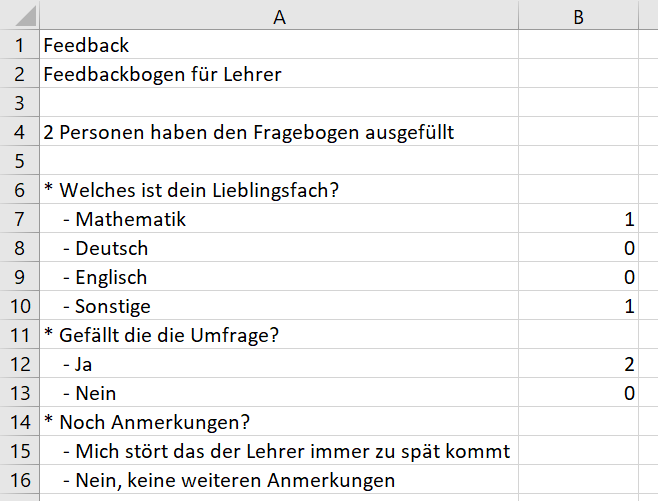
\includegraphics[width=0.5\textwidth]{pics/auswertung1.png}
    \caption{Auswertung}
    \label{fig:auswertungErgebnis1}
\end{figure}

Wie diese Auswertung umgsetzt wurde, wird in \ref{lst:auswertung1} gezeigt.
Mithilfe eines StringBuilders wurden alle nötigen Informationen zu einem String zusammengefügt und danach
mittels PrintWriter in das evaluation.csv File geschrieben. Es werden folgende Daten benötigt:
\begin{itemize}
  \item Name und Beschreibung vom aktuellen Fragebogen
  \item wie viele Transaktionscodes verwendet wurden, mit einem Verweis auf die aktuelle Umfrage
  \item für jede Frage jeweils
  \subitem den Namen
  \subitem die Antwortmöglichkeiten
  \subitem die Anzahl, wie oft eine Antwortmöglichkeit ausgewählt wurde
\end{itemize}
Es wird außerdem überprüft, ob eine Frage vom Typen Freetext ist. Ist dies der Fall, wird die Antwort dieser Frage
am Ende des Files angehängt.
\begin{lstlisting} [caption=Auswertung, label=lst:auswertung1]
  Survey survey = findById(surveyId);
  Questionnaire questionnaire = questionnaireRepository.findById(survey.questionnaire.id);
  List<Question> questions = questionRepository.getQuestionsByQuestionaireId(questionnaire.id);
  List<Transaction> transactions = transactionRepository.findBySurvey(survey);
  for (Transaction transaction : transactions) {
      if (transaction.isUsed){
          usedTransactions ++;
      }
  }
  File file = new File("evaluation.csv");
  try (PrintWriter writer = new PrintWriter("evaluation.csv")) {
      StringBuilder sb = new StringBuilder();
      sb.append(questionnaire.name);
      sb.append(questionnaire.description);
      sb.append(usedTransactions);
      sb.append(" Personen haben den Fragebogen ausgefuellt");
      for (Question question : questions) {
          sb.append(question.text);
          answers = answerRepository.findByQuestion(question);
          if (question.questiontype.equals(QuestionType.FREETEXT)){
              for (Answer answer : answers) {
                  sb.append("    - ");
                  sb.append(answer.answerText);
              }
          }else{
              answerOptions = answerOptionRepository.findByQuestionId(question.id);
              for (AnswerOption answerOption : answerOptions) {
                  chosenOptions = chosenOptionRepository.findByAnswerOption(answerOption);
                  sb.append("    - ");
                  sb.append(answerOption.text);
                  sb.append(": ");
                  sb.append(chosenOptions.size());
              }
          }
      }
      writer.write(sb.toString());
  } catch (FileNotFoundException e) {
      System.out.println(e.getMessage());
  }
\end{lstlisting}
Bei der zweiten Variante wurde sich dafür entschieden, pro Befragten den Wert der ausgewählten Antwortmöglichkeit
anzuzeigen. Wie so eine Auswertung aussehen kann sieht man in Abbildung \ref{fig:auswertungErgebnis2}.
\begin{figure}[h]
  \centering
    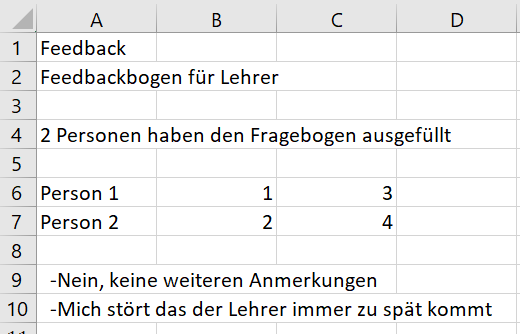
\includegraphics[width=0.5\textwidth]{pics/auswertung2.png}
    \caption{Auswertung}
    \label{fig:auswertungErgebnis2}
\end{figure}

Wie diese Auswertung umgsetzt wurde, wird in \ref{lst:auswertung2} gezeigt.
Mithilfe eines StringBuilders wurden alle nötigen Informationen zu einem String zusammengefügt und danach
mittels PrintWriter in das evaluation2.csv File geschrieben. Es werden folgende Daten benötigt:
\begin{itemize}
  \item Name und Beschreibung vom aktuellen Fragebogen
  \item wie viele Transaktionscodes verwendet wurden, mit einem Verweis auf die aktuelle Umfrage
  \item pro Transaktionscode, der für diese Umfrage verwendet wurde, den Wert der ausgewählten Antwortmöglichkeit, jeder Frage
\end{itemize}
Es wird außerdem überprüft, ob eine Frage vom Typen Freetext ist. Ist dies der Fall, wird die Antwort dieser Frage
am Ende des Files angehängt.
  \begin{lstlisting} [caption=Auswertung, label=lst:auswertung2]
      Survey survey = findById(surveyId);
      Questionnaire questionnaire = questionnaireRepository.findById(survey.questionnaire.id);
      List<Question> questions = questionRepository.getQuestionsByQuestionaireId(questionnaire.id);
      List<Transaction>transactions = transactionRepository.findBySurvey(survey);
      File file = new File("evaluation2.csv");
      try (PrintWriter writer = new PrintWriter("evaluation2.csv")) {
          StringBuilder sb = new StringBuilder();
          sb.append(questionnaire.name);
          sb.append(questionnaire.description);
          sb.append(usedTransactions);
          sb.append(" Personen haben den Fragebogen ausgefuellt");
        
          for (Transaction transaction : transactions) {
              answers = answerRepository.findByTransaction(transaction);
              count ++;
              sb.append("Person ");
              sb.append(count);
              sb.append(";");
              for (Answer answer : answers) {
                  chosenOptions = chosenOptionRepository.findByAnswer(answer);
                  for (ChosenOption chosenOption : chosenOptions) {
                      answerOpt = chosenOption.answerOption;
                      if (chosenOption.question.questiontype == QuestionType.FREETEXT){
                          sb.append("\n");
                          freetextAnswers.add(chosenOption.answer);
                      }else {
                          sb.append(" ");
                          sb.append(answerOpt.value);
                          sb.append(";");
                      }
                  }
              }
          }
          if (freetextAnswers.size() != 0){
              for (Answer answer : freetextAnswers) {
                  sb.append("\n");
                  sb.append("  -");
                  sb.append(answer.answerText);
              }
          }
          writer.write(sb.toString());
      } catch (FileNotFoundException e) {
          System.out.println(e.getMessage());
      }
      return file;
  }
  \end{lstlisting}
